\section{Machine Learning Analysis}
\label{sec:ml-analysis}

This section presents the machine learning analysis and addresses RQ1--RQ3.
We first apply unsupervised clustering to the daily feature panel from
Section~\ref{sec:feature-engineering} to identify recurring leverage and
looping strategy archetypes (RQ1, RQ2), and then train supervised models on
the same panel to test how far publicly observable on-chain state variables
can predict short-horizon rebalancing events and stressed risk states (RQ3).
Treating both within a single analysis allows the unsupervised archetypes to
be cross-checked against the supervised stress label, since the two are
derived independently of one another.

\subsection{Unsupervised Strategy Archetypes}
\label{sec:archetype-analysis}

This part addresses RQ1 and RQ2: what recurring leverage and looping
strategy archetypes can be identified among large yield-bearing token
holders, and which observable risk-management characteristics
differentiate them? We cluster the daily feature panel from
Section~\ref{sec:feature-engineering} with HDBSCAN to group whale-days by
behaviour rather than by wallet, characterise the resulting archetypes by
their leverage and risk profiles, and then cross-check them against the
stressed-state label introduced in Section~\ref{sec:ml-supervised}.

\subsubsection{Data and Features}
\label{sec:arch-data}

The analysis starts from the Morpho subset of the combined daily panel:
2{,}022 whale-day observations across 17 Morpho whales (W-1 through W-17).
We restrict it to the 1{,}750 days on which a whale holds an open,
actively looped position, that is, days with a non-missing \texttt{ltv},
\texttt{carry\_spread}, and \texttt{carry\_spread\_levered}; days with no
open debt carry no looping behaviour to cluster. Each retained day is
described by eleven features
spanning leverage (\texttt{ltv}, \texttt{loop\_depth},
\texttt{distance\_to\_liq}), leverage dynamics (\texttt{ltv\_vol\_7d},
\texttt{ltv\_vol\_14d}, \texttt{ltv\_lag\_7}), rebalancing behaviour
(\texttt{rebal\_freq\_7d}, \texttt{rebal\_freq\_30d},
\texttt{days\_since\_rebalance}), and carry (\texttt{carry\_spread},
\texttt{carry\_spread\_levered}). Missing values are imputed with feature
medians and all features are standardised so that HDBSCAN does not treat
a high-variance feature as more important purely because of its scale.

As Figure~\ref{fig:mean-ltv-per-whale} shows, the whales operate at very
different baseline leverage levels, which motivates both the feature
standardisation and the balancing step described below.

\begin{figure}[t]
\centering
\includegraphics[width=0.8\textwidth]{figures/mean-ltv-per-whale.png}
\caption{Mean LTV per whale on days with an open debt position. The
whales operate at markedly different baseline leverage levels, from
near-fully-levered wallets to more conservative loopers.}
\label{fig:mean-ltv-per-whale}
\end{figure}

\subsubsection{Clustering Method and Setup}
\label{sec:arch-setup}

We use HDBSCAN, a density-based clustering algorithm that groups points
in dense regions of feature space and labels sparse points as noise
rather than forcing every observation into a cluster. This suits our
setting, where many whale-days fall into a few recurring behavioural
modes while transitional or idle days do not. We visualise the clusters
by projecting the eleven standardised features onto their first two
principal components (PCA), which is used only for display and not for
the clustering itself.

A baseline fit on the full panel (\texttt{min\_cluster\_size}$=15$,
\texttt{min\_samples}$=5$) returns eight clusters together with roughly
$29\%$ noise, but the clusters are largely whale-specific: because some
whales contribute many more days than others, the baseline structure
reflects \emph{who} has the most days as much as \emph{how} they behave
(Figure~\ref{fig:pca-baseline}). To recover shared strategy archetypes rather than per-wallet groups, we
balance the fit by keeping only whales with at least eight active looping
days (excluding W-17 with a single day) and drawing eight days from each
remaining whale ($8 \times 16 = 128$ rows, \texttt{random\_state}$=42$).
A parameter sweep on this balanced sample gives three dense clusters at
\texttt{min\_cluster\_size}$=8$ and \texttt{min\_samples}$=3$, which we
adopt.

To label every day rather than only the balanced sample, we assign all
1{,}750 days to the nearest cluster centroid and flag days beyond the
$95$th percentile of centroid distance as outliers. The three dense
clusters plus this outlier group give four archetypes, named from their
feature profiles rather than fixed cluster IDs.

\begin{figure}[t]
\centering
\includegraphics[width=0.48\textwidth]{figures/pca-by-baseline-cluster.png}
\hfill
\includegraphics[width=0.48\textwidth]{figures/pca-by-whale.png}
\caption{PCA projection of whale-days from the baseline (unbalanced) fit,
coloured by HDBSCAN cluster (left) and by whale (right). The cluster
boundaries largely coincide with wallet identity, which shows that the
unbalanced fit recovers whale-specific groups rather than shared strategy
archetypes and motivates the balanced fit in
Section~\ref{sec:arch-setup}.}
\label{fig:pca-baseline}
\end{figure}

\subsubsection{Identified Archetypes}
\label{sec:archetypes}

The four archetypes and their mean risk profiles are reported in
Table~\ref{tab:archetypes} and visualised in
Figure~\ref{fig:pca-by-archetype}. The per-whale composition of each
archetype is given in Table~\ref{tab:archetype-membership}.

Answering RQ2, the three looping archetypes are differentiated, in order
of importance, by leverage level, loop depth, rebalancing cadence, and
levered carry, as the mean profiles in Table~\ref{tab:archetypes} show.
The characteristics of each mode can be stated explicitly as follows.

\emph{Stale / light loop} runs a low LTV (around $0.34$, roughly
$2\times$ leverage) with a shallow loop and a wide liquidation buffer
(around $0.55$), rebalances infrequently (about every $35$ days), and
earns a low levered carry. It is the conservative, lightly geared mode.

\emph{Moderate leverage} runs a mid-range LTV (around $0.67$, roughly
$7\times$) with active maintenance (about $1$ day since last
rebalance) and medium levered carry. These are active risk managers.

\emph{High-LTV hold} runs a high LTV (around $0.90$, roughly $13\times$)
with a deep loop but only a thin buffer (around $0.04$), holds the
position with infrequent rebalancing (about every $49$ days), and earns
the highest levered carry. It is aggressive, set-and-forget looping.

The \emph{idle / outlier} group collects near-zero-LTV and transitional
days (LTV around $0.28$) that are geometrically distant from all
centroids or represent unwound positions. High-LTV hold and moderate
leverage are separated mainly by leverage intensity and maintenance
cadence rather than by carry alone.

\begin{table}[t]
\centering
\small
\caption{Strategy archetypes and mean risk profiles over the 1{,}750
assigned whale-days. Loop depth is the effective leverage multiple and
distance to liquidation (\texttt{dist.\ to liq.}) is the remaining LTV
buffer before the position becomes liquidatable.}
\label{tab:archetypes}
\begin{tabular}{lcccccc}
\hline
Archetype & Days & \% & Mean LTV & Loop depth & Dist.\ to liq. & Days since rebal. \\
\hline
stale / light loop & 667 & 38 & 0.34 & 2.3 & 0.55 & 35 \\
high-LTV hold & 593 & 34 & 0.90 & 12.9 & 0.04 & 49 \\
moderate leverage & 402 & 23 & 0.67 & 7.4 & 0.24 & 1 \\
idle / outlier & 88 & 5 & 0.28 & 2.3 & 0.66 & 4 \\
\hline
\end{tabular}
\end{table}

\begin{table}[t]
\centering
\small
\caption{Archetype membership as a percentage of each whale's days
(selected whales; full table in repository).}
\label{tab:archetype-membership}
\begin{tabular}{lcccc}
\hline
Whale & stale / light & high-LTV hold & idle / outlier & moderate \\
\hline
W-2 & 0.0 & 92.0 & 8.0 & 0.0 \\
W-3 & 32.4 & 2.9 & 8.6 & 56.1 \\
W-6 & 0.0 & 100.0 & 0.0 & 0.0 \\
W-11 & 70.9 & 1.6 & 1.3 & 26.2 \\
W-12 & 0.0 & 100.0 & 0.0 & 0.0 \\
W-4 & 73.1 & 0.0 & 0.0 & 26.9 \\
W-5 & 79.4 & 0.0 & 0.0 & 20.6 \\
\hline
\end{tabular}
\end{table}

\begin{figure}[t]
\centering
\includegraphics[width=0.9\textwidth]{figures/pca-by-archetype.png}
\caption{PCA projection of whale-days coloured by assigned archetype.
The three dense looping archetypes separate on leverage, loop depth, and
rebalancing cadence; the idle / outlier group collects unwound or
transitional days.}
\label{fig:pca-by-archetype}
\end{figure}

\subsubsection{Findings}
\label{sec:arch-findings}

Taken together, the clustering gives a clear answer to RQ1 and RQ2: a
small number of recurring looping modes exist, and they are differentiated
primarily by leverage, loop depth, and rebalancing cadence.

\paragraph{Four recurring modes, not seventeen whale types.}
After balancing across 17 Morpho whales, whale-days collapse into three
dense behavioural clusters plus an idle / outlier group. The archetypes
describe \emph{how} whales loop rather than \emph{which} wallet they are.

\paragraph{Whales are mixed strategists.}
Only five of seventeen whales are \emph{pure} strategists ($\geq 80\%$ of
days in one archetype): W-2, W-6, and W-12 (high-LTV hold), W-15
(moderate leverage), and W-17 (stale / light loop). W-3 in particular
spreads across all four archetypes (56\% moderate), which indicates that
strategy is better described as mode-switching over time than as a fixed
per-wallet type.

\paragraph{Moderate leverage masks day-level heterogeneity.}
The moderate-leverage centroid sits between conservative and aggressive
modes, but individual days within it scatter: W-4 and W-5 contribute
mostly stale / light loop days, while W-3 mixes light- and core-moderate
assignments (LTV below vs.\ above $0.6$). Cluster averages can therefore
understate how far a mixed strategist moves between low- and high-risk
states.

\subsubsection{Stress by Archetype: a Sanity Check}
\label{sec:stress-by-archetype}

Having characterised and summarised the archetypes, we close the
unsupervised analysis by checking them against an independent risk
outcome, which also forms the bridge into the supervised prediction that
follows. The join serves as a sanity check on the archetypes. Two things
were done independently: first, the clustering of
Section~\ref{sec:archetype-analysis} grouped whale-days purely by
behaviour, with no access to any risk-outcome label; second, the
supervised \texttt{stressed\_state} label of
Section~\ref{sec:ml-supervised} flags days on which health factor falls
to $1.05$ or below (a fixed, cross-whale threshold). Having built the two
separately, we can now ask whether behaviourally risky archetypes also
accumulate more stressed days. We join the label onto the archetype panel
by \texttt{whale\_id} and \texttt{date} (all 1{,}750 days match) and
report the stressed share per archetype
(Table~\ref{tab:stress-by-archetype},
Figure~\ref{fig:stress-by-archetype}).

\begin{table}[t]
\centering
\caption{Stressed share of days per archetype (health factor $\leq 1.05$).}
\label{tab:stress-by-archetype}
\begin{tabular}{lcc}
\hline
Archetype & Days & Stressed \% \\
\hline
high-LTV hold & 593 & 63.7 \\
moderate leverage & 402 & 34.6 \\
idle / outlier & 88 & 13.6 \\
stale / light loop & 667 & 5.1 \\
\hline
\end{tabular}
\end{table}

\begin{figure}[t]
\centering
\includegraphics[width=0.9\textwidth]{figures/stress-by-archetype.png}
\caption{Stressed share of days per archetype under the fixed health-factor
threshold (HF $\leq 1.05$). Risk rises monotonically from stale / light
loop to high-LTV hold.}
\label{fig:stress-by-archetype}
\end{figure}

Under the shared threshold the stressed share rises with leverage
intensity: high-LTV hold (63.7\%) and moderate leverage (34.6\%) sit
above stale / light loop (5.1\%) and idle / outlier days (13.6\%). Because
the archetypes were built without the stress label, this ordering is an
independent check that the clusters capture genuine risk structure. The
main caveat, discussed in Section~\ref{sec:discussion}, is that some
archetypes remain whale-dominated and the sample is restricted to Morpho
loopers; held-out-whale validation of the supervised models is left as
future robustness work.





\subsection{Supervised Prediction of Rebalancing and Stress}
\label{sec:ml-supervised}

This part addresses RQ3: to what extent can on-chain state variables
predict short-horizon rebalancing events and stressed risk states? We
train supervised models on the daily feature panel from
Section~\ref{sec:feature-engineering} and use them to test whether
publicly observable on-chain signals carry enough information to
anticipate whale behaviour and risk. We frame this as two separate
binary prediction tasks: whether a whale will rebalance its position on a
given day (Model~A), and whether a whale is in a stressed risk state on a
given day (Model~B).

\subsubsection{Data and Labels}
\label{sec:ml-data}

The analysis uses the daily feature panel of 2{,}507 whale-day
observations across 24 whales (W-1 through W-24), spanning
2024-03-29 to 2026-06-27. Each observation carries the leverage,
risk, behavioural, and carry features described in
Section~\ref{sec:feature-engineering}.

The target for Model~A, \texttt{rebalancing}, is already present in the
panel: it flags any day on which a supply, withdraw, borrow, or repay
event occurred. Rebalancing days are the minority class, accounting for
$14.8\%$ of observations (371 of 2{,}507 days).

The target for Model~B, \texttt{stressed\_state}, is constructed during
exploratory analysis. We label a whale-day as stressed if its health
factor falls to $1.05$ or below. We use this fixed threshold rather than
a per-whale percentile because health factor has a fixed real-world
meaning: $1.0$ is liquidation. A per-whale percentile approach (such as
marking each whale's worst $30\%$ of days) would compare each whale only
to itself, making a whale that lives permanently near $1.0$ look no
riskier than one that always stays safely above $1.4$, since both would
show a similar stressed rate. A fixed threshold ensures that the label
reflects real proximity to liquidation and is comparable across all
whales.

\subsubsection{Exploratory Analysis}
\label{sec:ml-eda}

Before building the prediction models, we examine the distribution of
health factor, distance to liquidation, stressed rate, and rebalancing
behaviour across all 24 whales.

\paragraph{Health factor and distance to liquidation.}
Most whales cluster tightly, with mean health factor between roughly
$1.0$ and $1.1$ and minimums close to $1.0$. A few stand apart.
W-11 is the largest outlier, with a mean health factor of approximately
$2.0$ and a maximum above $4.7$; it mostly holds a very safe position
but has experienced sharp dips. W-16 and W-14 also run higher than
average, with means around $1.4$ and $1.25$. At the risky end, W-1 and
W-12 keep mean health factors close to $1.01$, meaning they operate with
almost no buffer above liquidation at any point.

The distance-to-liquidation metric shows the same broad structure. W-11
and W-16 have the highest average buffers (both above $0.5$), though
their minimums still drop to around $0.06$ to $0.08$. W-3 and W-13
show a high mean but very low minimum pattern: their average buffers are
roughly $0.34$ and $0.39$, but minimums fall close to zero, indicating
swings between safe periods and sudden brushes with liquidation. W-1
sits at the opposite end, with both mean and minimum close to zero.

Across both metrics, the whales split into three broad groups: a small
set with high average safety but occasional risky dips (W-11, W-16, W-3,
W-13), a set of steady conservative operators that never approach
liquidation (W-4, W-5, W-8, W-24), and whales that sit close to
liquidation almost constantly (W-1, W-12).

\paragraph{Stressed rate under the fixed threshold.}
Under the $1.05$ threshold, the overall stressed rate is $28.9\%$
(725 of 2{,}507 days). The rate varies widely across whales. W-12 and
W-1 are stressed on more than $95\%$ of their days, while W-18 and W-7
sit at $90.9\%$ and $81.0\%$. At the other end, nine whales (W-4, W-5,
W-8, W-11, W-16, W-17, W-19, W-23, W-24) never drop to $1.05$ or below.
The remaining whales fall in between, with stressed rates ranging from
about $13\%$ up to $71\%$.

\paragraph{Rebalancing behaviour.}
Overall, whales rebalanced on 371 of 2{,}507 days ($14.8\%$). The most
active rebalancers are W-15 and W-23 (both $55.6\%$), W-16 ($52.6\%$),
W-3 ($47.5\%$), and W-7 ($44.8\%$). Most other whales rebalance on
fewer than $15\%$ of their days. W-17 shows $100\%$ but has only a
single observation, so this number should not be interpreted as
meaningful.

\subsubsection{Models and Setup}
\label{sec:ml-setup}

For each task we split the data into stratified training and test sets
($70/30$) and fit two models. A logistic regression serves as an
interpretable linear baseline, and a gradient-boosted tree model
(XGBoost) serves as the main nonlinear model. This split estimates
predictive signal within the panel; held-out-whale validation (training
on some whales and testing on others) is recommended as future
robustness work. XGBoost builds an ensemble
of small decision trees in sequence, where each tree corrects the errors
of the ones before it; it is well suited to imbalanced tabular datasets
such as ours. To interpret its predictions we use SHAP (SHapley Additive
exPlanations), which attributes each prediction to its input features and
reports how much each variable pushed the prediction up or down. SHAP is
what lets us move from a yes/no prediction to a statement about
\emph{which} on-chain variables drive whale behaviour and by how much,
which is what RQ3 asks.

To handle the class imbalance in the rebalancing task, we weight the
positive class using XGBoost's \texttt{scale\_pos\_weight}. For the
stressed-state model we lower the decision threshold from the default
$0.5$ to $0.3$; we compare both thresholds for both classifiers and
justify this choice in Section~\ref{sec:model-stressed}.

\paragraph{Avoiding data leakage.}
We exclude any feature that encodes the answer it is meant to predict.
Model~A omits the rebalancing-frequency and recency features
(\texttt{rebal\_freq\_7d}, \texttt{rebal\_freq\_30d},
\texttt{days\_since\_rebalance}), since these are derived from the
rebalancing flag that forms the target.

Model~B required more careful exclusion. The initial feature set included
\texttt{ltv} and its lagged variants, \texttt{health\_factor},
\texttt{distance\_to\_liq}, and \texttt{loop\_depth}. The first training
run produced a ROC-AUC of $1.000$, a clear sign of leakage. Checking the
raw values confirmed the cause: \texttt{ltv} above roughly $0.87$ almost
perfectly separated stressed from non-stressed days, and
\texttt{loop\_depth} above $8$ did the same. Both features were removed,
along with \texttt{ltv\_lag\_1}, \texttt{ltv\_lag\_3}, and
\texttt{ltv\_lag\_7}, since \texttt{health\_factor} (which defines
\texttt{stressed\_state}) is built directly from \texttt{ltv}. A second,
smaller leak was then found: \texttt{collateral\_balance} and
\texttt{borrow\_balance} let XGBoost reach a ROC-AUC of $0.993$, a much
larger jump over logistic regression than expected. Trees can exploit
hidden cutoffs in raw numbers more easily than a linear model, so a leak
that logistic regression missed still showed up in XGBoost. Removing
these two balance features brought XGBoost back to a realistic $0.977$,
close to logistic regression's $0.971$, confirming the leak was resolved.

The final exclusion list for Model~B therefore covers: \texttt{ltv},
\texttt{ltv\_lag\_1}, \texttt{ltv\_lag\_3}, \texttt{ltv\_lag\_7},
\texttt{health\_factor}, \texttt{distance\_to\_liq},
\texttt{loop\_depth}, \texttt{collateral\_balance\_usd},
\texttt{borrow\_balance\_usd}, \texttt{liquidation\_threshold},
\texttt{collateral\_balance}, and \texttt{borrow\_balance}.

\subsubsection{Model A: Predicting Rebalancing}
\label{sec:model-rebalancing}

Model~A predicts whether a whale will rebalance on a given day using 11
features: current and lagged LTV (\texttt{ltv}, \texttt{ltv\_lag\_1},
\texttt{ltv\_lag\_3}, \texttt{ltv\_lag\_7}), LTV volatility
(\texttt{ltv\_vol\_7d}, \texttt{ltv\_vol\_14d}), distance to liquidation,
health factor, carry spread (raw and levered), and loop depth.
After dropping rows with missing features, the modelling set is 1{,}475
rows; a stratified $70/30$ split gives 1{,}032 training and 443 test
observations. Results are reported in Table~\ref{tab:model-a}.

\begin{table}[t]
\centering
\caption{Model~A: rebalancing prediction.}
\label{tab:model-a}
\begin{tabular}{lccc}
\hline
Model & ROC-AUC & Recall & Precision \\
\hline
Logistic Regression & 0.828 & 0.69 & 0.36 \\
XGBoost             & 0.876 & 0.71 & 0.41 \\
\hline
\end{tabular}
\end{table}

XGBoost improves on every measure compared to the baseline. It catches
slightly more rebalancing days (46 of 65 versus 45 of 65), makes fewer
false alarms (65 versus 79), and achieves a stronger ROC-AUC ($0.876$
versus $0.828$). The improvement is modest but consistent across the
board.

To interpret the nonlinear model we examine its gain-based feature
importance (Figure~\ref{fig:rebal-gain}) and the SHAP summary of its
predictions (Figure~\ref{fig:rebal-shap}). The two views agree on the
substance: rebalancing is driven mainly by leverage volatility and
accumulated leverage history rather than by present-day risk snapshots.
\texttt{ltv\_vol\_7d} ($65.2$) is the most important feature by a small
margin, followed closely by \texttt{ltv\_lag\_7} ($61.5$) and
\texttt{ltv} ($45.3$). The remaining LTV features
(\texttt{ltv\_vol\_14d}, \texttt{ltv\_lag\_1}, \texttt{ltv\_lag\_3}) all
contribute meaningfully. In contrast, the carry features rank near the
bottom (\texttt{carry\_spread\_levered} at $19.5$, \texttt{carry\_spread}
at $9.8$), and \texttt{health\_factor} ranks lowest at $6.9$. Two
features, \texttt{distance\_to\_liq} and \texttt{loop\_depth}, were never
selected by any tree in the model.

The SHAP summary confirms the direction of these effects. Low LTV
volatility (blue dots) clusters tightly near zero, meaning stable
leverage rarely leads to rebalancing, while high lagged LTV pushes the
model towards predicting a rebalance. In other words, whales respond to
sustained leverage buildup over several days, combined with recent
volatility, rather than to a single day's risk reading or yield signal.

\begin{figure}[t]
\centering
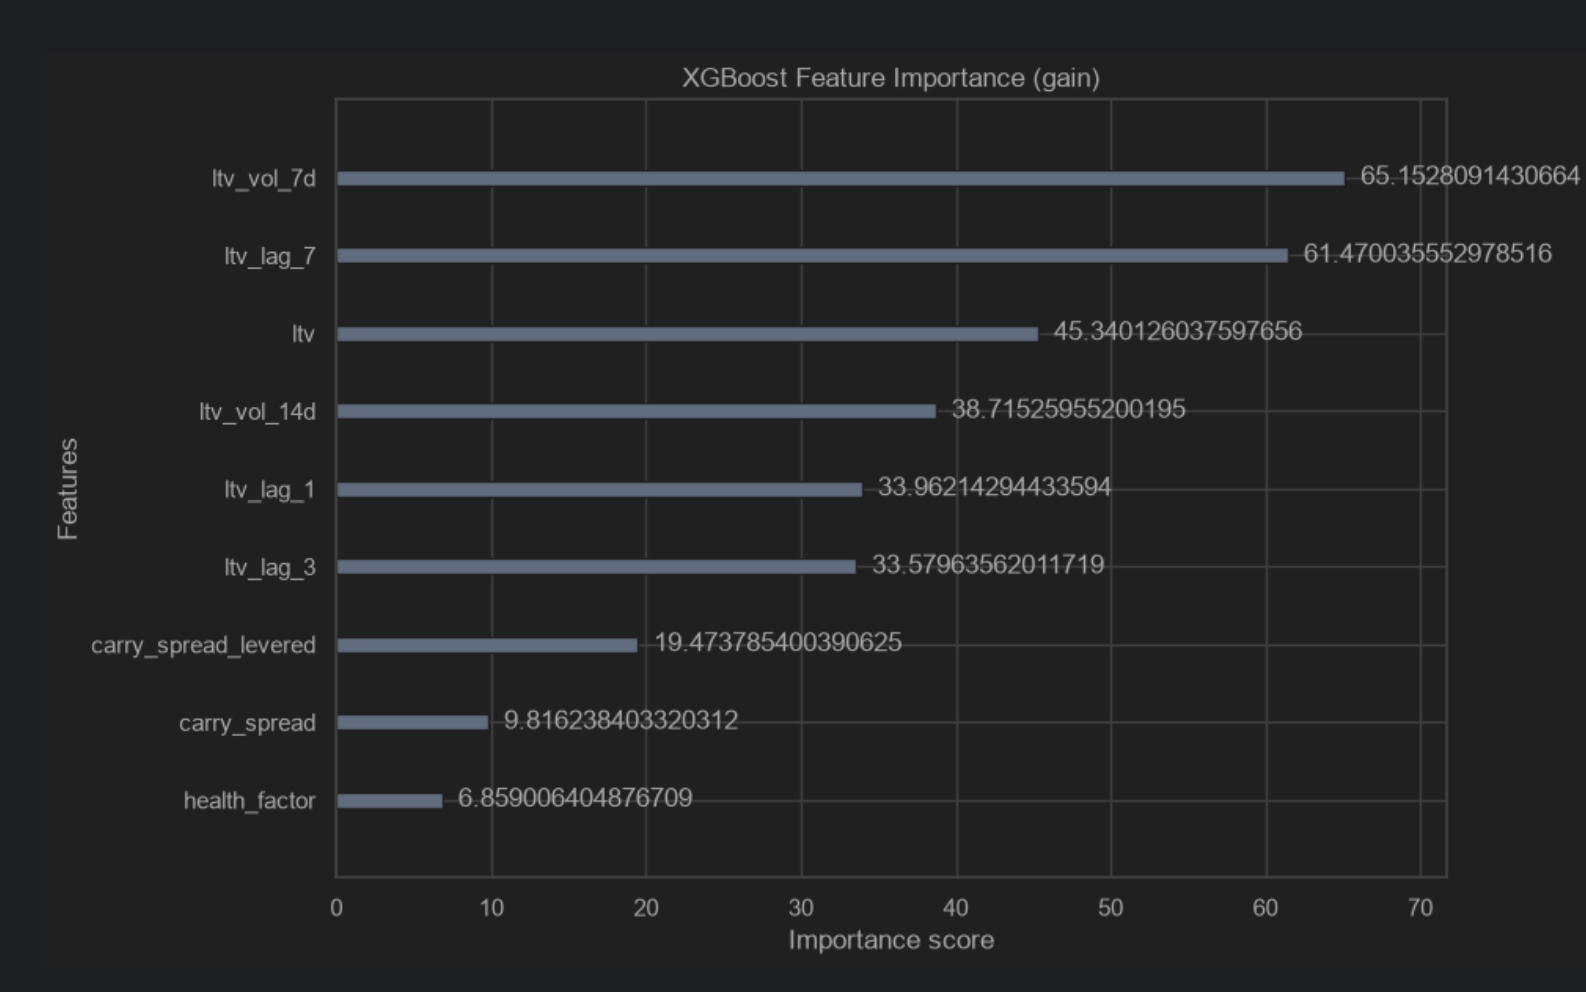
\includegraphics[width=0.9\textwidth]{figures/supervised/rebalance-xgb-feature-importance.png}
\caption{Gain-based feature importance for the XGBoost rebalancing model.
Bars show each feature's total gain (the improvement it contributes to
the split criterion) summed across all trees. LTV volatility
(\texttt{ltv\_vol\_7d}) and lagged LTV (\texttt{ltv\_lag\_7}) rank
highest; carry features and health factor rank lowest. Two features
(\texttt{distance\_to\_liq}, \texttt{loop\_depth}) were never used by any
tree and do not appear in the chart.}
\label{fig:rebal-gain}
\end{figure}

\begin{figure}[t]
\centering
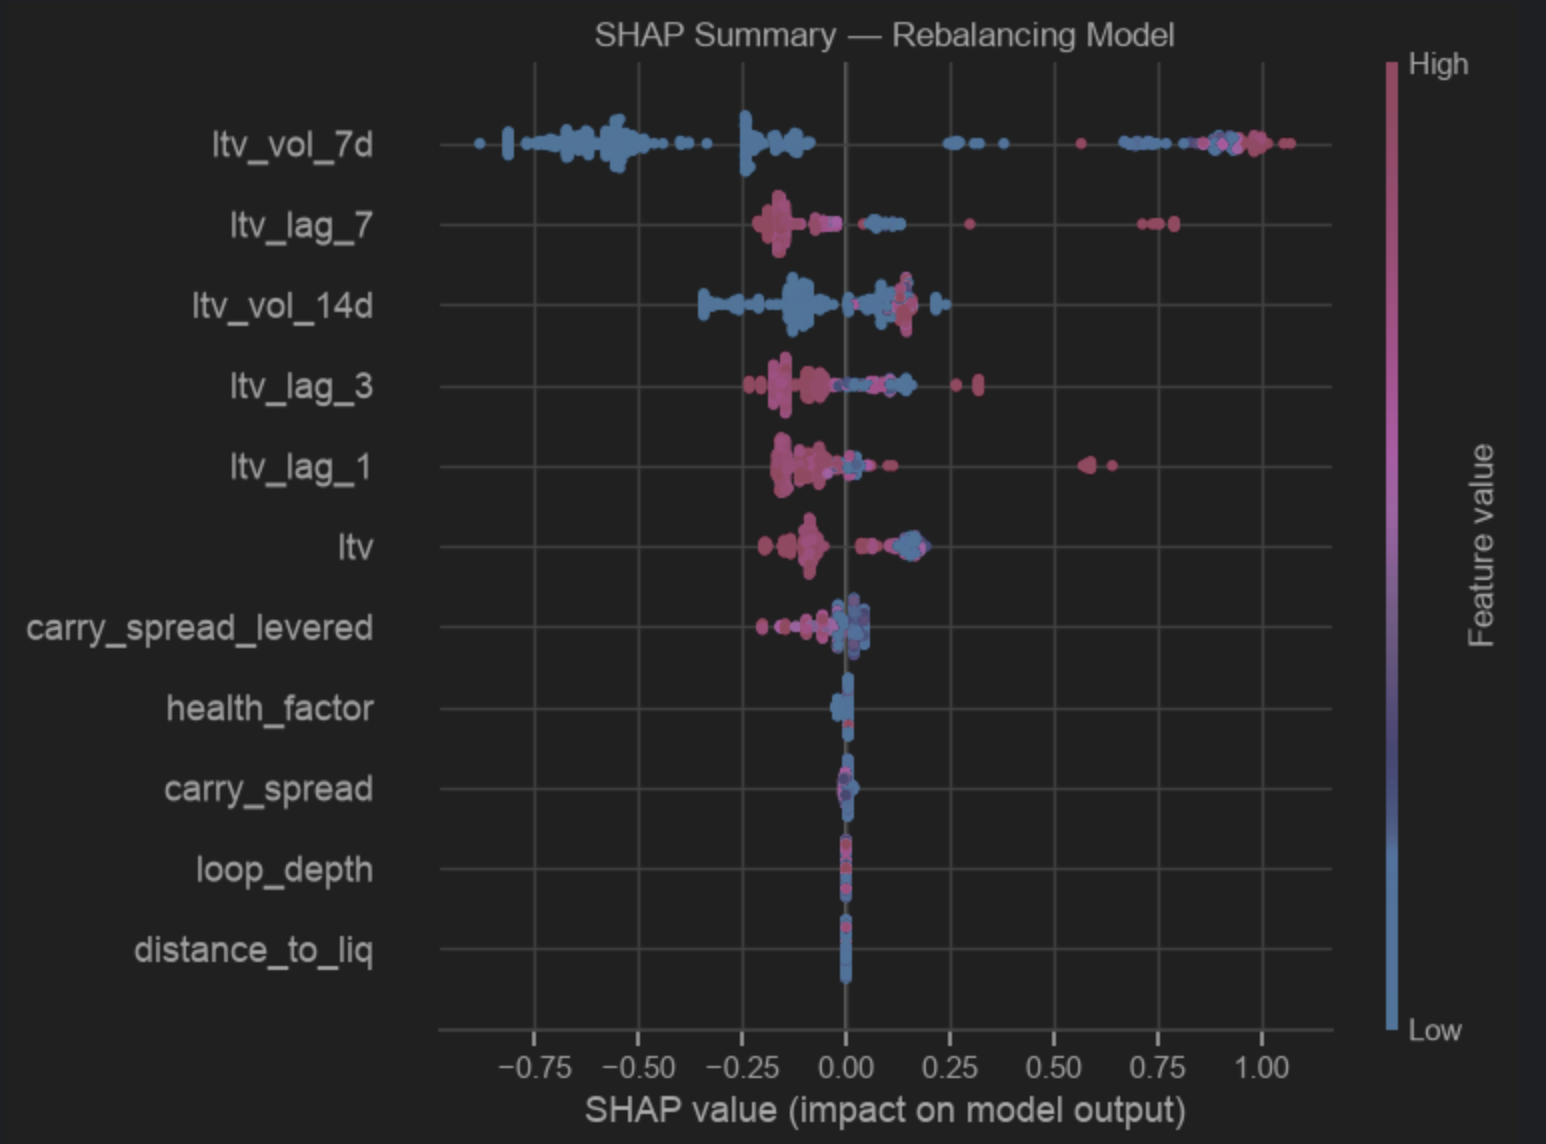
\includegraphics[width=0.9\textwidth]{figures/supervised/rebalance-shap.png}
\caption{SHAP summary for the XGBoost rebalancing model. Each point is a
whale-day; its horizontal position is the feature's signed contribution
to the predicted log-odds of rebalancing, and colour encodes the feature
value (red high, blue low). Features are ordered by mean absolute SHAP
value. High lagged LTV and high short-window LTV volatility push
predictions towards rebalancing, while the carry features and health
factor contribute little.}
\label{fig:rebal-shap}
\end{figure}

\subsubsection{Model B: Predicting Stressed States}
\label{sec:model-stressed}

Model~B predicts whether a whale is in a stressed risk state on a given
day using 9 features: LTV volatility (\texttt{ltv\_vol\_7d},
\texttt{ltv\_vol\_14d}), carry spread (raw and levered), yield and
interest rate variables (\texttt{ybt\_apy}, \texttt{borrow\_rate},
\texttt{supply\_rate}), and token prices (\texttt{collateral\_price},
\texttt{borrow\_price}). The feature set differs from Model~A because
several variables that are safe to use when predicting rebalancing
(such as \texttt{ltv}, \texttt{health\_factor}, and
\texttt{loop\_depth}) are too closely tied to the definition of
\texttt{stressed\_state} and would cause data leakage, as described in
Section~\ref{sec:ml-setup}.

After dropping rows with missing features, the modelling set is 2{,}088
rows; a stratified $70/30$ split gives 1{,}460 training and 628 test
observations. We evaluate both classifiers at two decision thresholds,
the default $0.5$ and a lowered $0.3$, and report all four
configurations in Table~\ref{tab:model-b}.

\begin{table}[t]
\centering
\caption{Model~B: stressed-state prediction across both classifiers and
both decision thresholds. ROC-AUC is threshold-independent and so repeats
within each model. The selected configuration (XGBoost at $t=0.3$) is
shown in bold.}
\label{tab:model-b}
\begin{tabular}{llcccc}
\hline
Model & $t$ & ROC-AUC & Recall & Precision & Accuracy \\
\hline
Logistic Regression & 0.5 & 0.971 & 0.95 & 0.75 & 0.89 \\
Logistic Regression & 0.3 & 0.971 & 0.98 & 0.67 & 0.84 \\
XGBoost             & 0.5 & 0.977 & 0.82 & 0.93 & 0.92 \\
\textbf{XGBoost}    & \textbf{0.3} & \textbf{0.977} & \textbf{0.90} & \textbf{0.81} & \textbf{0.90} \\
\hline
\end{tabular}
\end{table}

\paragraph{Choice of decision threshold.}
By default a classifier labels a day as stressed only when its predicted
probability exceeds $0.5$. We lower this threshold to $0.3$ so that the
model raises a flag whenever it is at least $30\%$ confident, catching
more stressed days at the cost of some false alarms. This trade-off is
deliberate: in a risk-monitoring setting a missed stressed day is far
more costly than a false alarm, since an unflagged stressed whale may
proceed to liquidation, whereas a false alarm merely prompts an
unnecessary check. Lowering the threshold therefore prioritises recall,
which is the quantity that matters most for this task.

\paragraph{Choice of model.}
The two classifiers behave differently at the lower threshold. Logistic
regression at $t=0.3$ achieves the highest recall ($0.98$) but at the
cost of precision: only $0.67$ of its stress predictions are correct, and
accuracy falls to $0.84$. XGBoost at $t=0.3$ reaches a recall of $0.90$
(catching 180 of 199 stressed days, missing only 19) while retaining a
precision of $0.81$ (with 42 false alarms out of 429 non-stressed days)
and an accuracy of $0.90$, alongside a stronger ROC-AUC ($0.977$ versus
$0.971$). XGBoost therefore identifies stressed states from their
underlying structure rather than by widening its positive predictions
indiscriminately, and we adopt it at $t=0.3$ as the final stressed-state
model.

With this configuration fixed, the gain-based feature importance
(Figure~\ref{fig:stress-gain}) and the SHAP summary
(Figure~\ref{fig:stress-shap}) show that stress is driven primarily by
yield and interest rate conditions rather than by leverage alone.
\texttt{ybt\_apy} ($89.3$) ranks first, followed closely by
\texttt{carry\_spread} ($84.5$), \texttt{supply\_rate} ($82.8$), and
\texttt{carry\_spread\_levered} ($71.8$). LTV volatility
(\texttt{ltv\_vol\_7d} at $69.6$, \texttt{ltv\_vol\_14d} at $41.3$) and
\texttt{borrow\_rate} ($40.2$) also contribute, but less than the yield
features. \texttt{collateral\_price} ($32.6$) and
\texttt{borrow\_price} ($28.2$) rank lowest, though neither is close to
zero. Importantly, no single feature dominates the way that
\texttt{ltv} or \texttt{loop\_depth} did in the leaking models, which
supports the conclusion that this result is genuine.

The SHAP summary confirms the direction of these effects.
\texttt{carry\_spread\_levered} has the widest spread (roughly $-1.5$ to
$1.5$): high values push strongly toward stress, while low values push
away from it. For \texttt{ybt\_apy} and \texttt{supply\_rate}, low values
(blue dots) push toward stress, consistent with the idea that falling
yields make a position more vulnerable. The volatility features show a
smaller rightward pull, meaning they add some signal but less than the
yield features.

\begin{figure}[t]
\centering
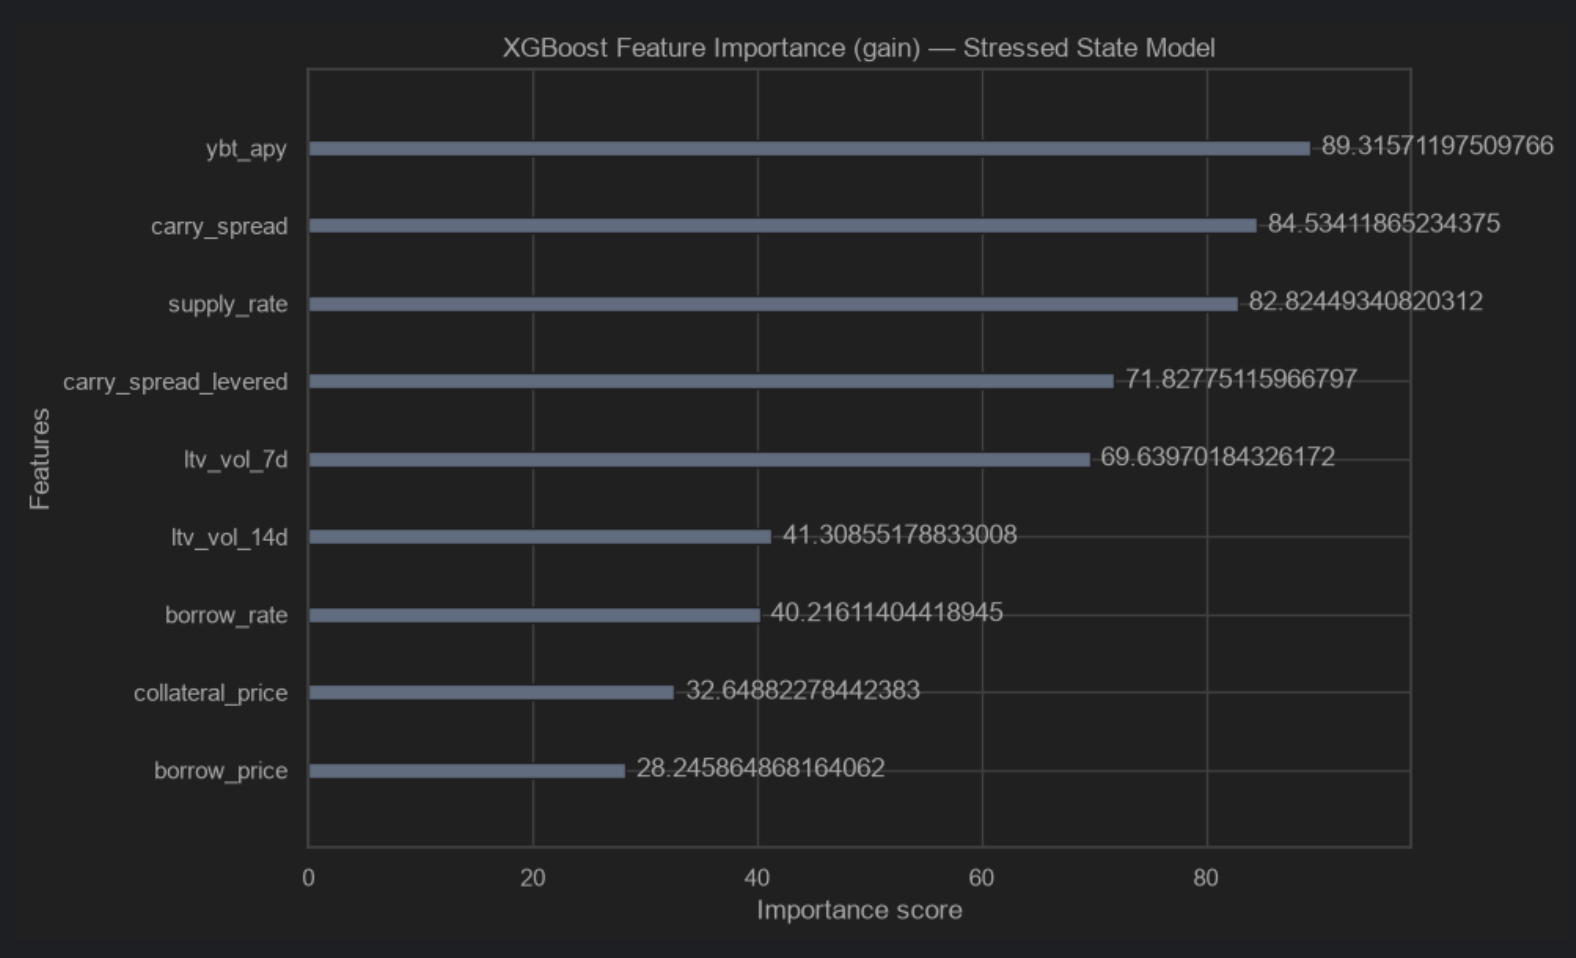
\includegraphics[width=0.9\textwidth]{figures/supervised/stress-feature-importance.png}
\caption{Gain-based feature importance for the XGBoost stressed-state
model. Bars show each feature's total gain summed across all trees. Yield
and rate features (\texttt{ybt\_apy}, \texttt{carry\_spread},
\texttt{supply\_rate}) rank highest; price features rank lowest. No
single feature dominates, and the label-defining features
(\texttt{health\_factor}, \texttt{distance\_to\_liq}) along with other
leaking variables are excluded.}
\label{fig:stress-gain}
\end{figure}

\begin{figure}[t]
\centering
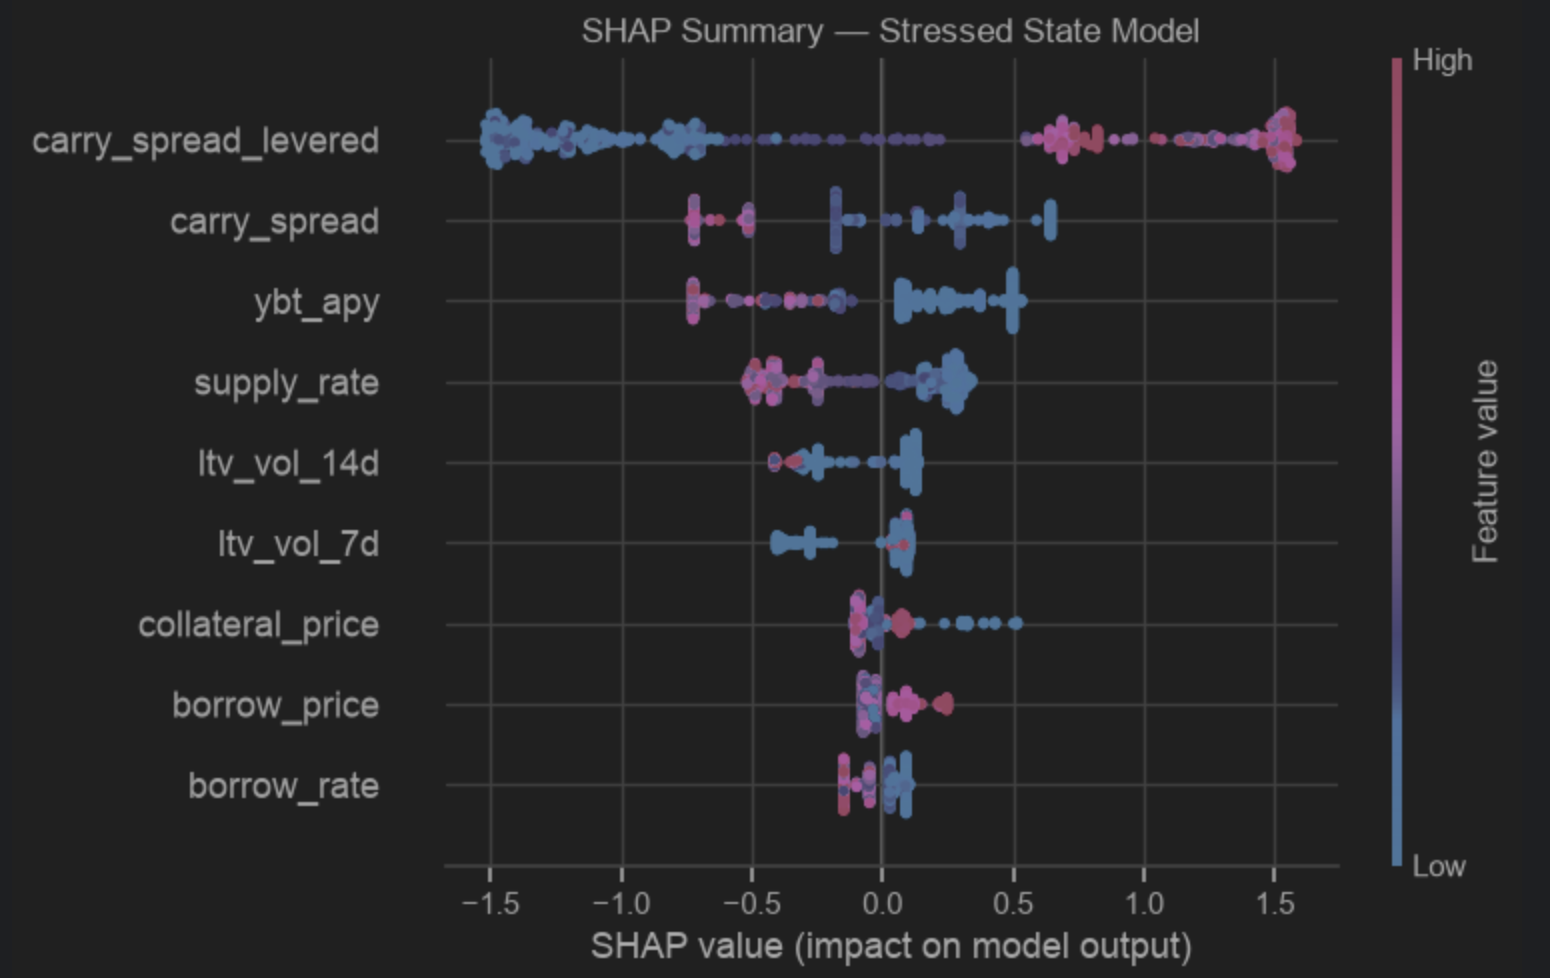
\includegraphics[width=0.9\textwidth]{figures/supervised/stress-shap.png}
\caption{SHAP summary for the XGBoost stressed-state model. Each point is
a whale-day; its horizontal position is the feature's signed contribution
to the predicted log-odds of being stressed, and colour encodes the
feature value (red high, blue low). Features are ordered by mean absolute
SHAP value. \texttt{carry\_spread\_levered} has the widest spread; low
yield (\texttt{ybt\_apy}) and low supply rate push predictions toward
stress.}
\label{fig:stress-shap}
\end{figure}

\subsubsection{Findings}
\label{sec:ml-findings}

Taken together, the two models give a clear answer to RQ3: on-chain state
variables can predict both rebalancing and stress, but through different
mechanisms.

\paragraph{Rebalancing is a delayed response.}
Whales do not rebalance the moment risk rises. The strongest predictors
of rebalancing are LTV volatility over the past week and lagged LTV
values rather than the current level, which indicates that operators
watch leverage accumulate and fluctuate over several days before acting.
Rebalancing therefore looks like a considered decision rather than a
panic reaction.

\paragraph{Stress tracks yield and rate conditions.}
The stressed-state model achieves strong detection (ROC-AUC of $0.977$,
recall of $0.90$ at threshold $0.3$) using only yield, rate, volatility,
and price features, without any direct leverage or structural variables.
The dominant predictors are \texttt{ybt\_apy}, \texttt{carry\_spread},
and \texttt{supply\_rate}. This suggests that a whale is more likely to
be in a stressed state when the yield it earns drops too close to its
borrowing cost, rather than simply when leverage is high. Stress in this
dataset looks less like ``leverage got too high'' and more like ``the
position stopped being worth the risk.''

\paragraph{Leverage volatility matters for both, but plays different
roles.}
In the rebalancing model, \texttt{ltv\_vol\_7d} is the single most
important feature. In the stressed-state model, it still matters but
ranks behind the yield and rate features. This suggests that volatility
is more of a trigger for action (rebalancing) than a marker of danger
(stress) in this dataset.

\paragraph{The broader picture.}
Whales appear to watch leverage build up over time before deciding to
rebalance, while their stressed state on any given day is shaped more
by yield and rate conditions than by leverage swings alone. On-chain
data captures both of these patterns clearly, which means that DeFi
leverage risk can likely be monitored, and to some extent anticipated,
in real time using only publicly available blockchain data. This is
directly relevant to on-chain risk monitoring and protocol parameter
calibration.